\documentclass[12pt,a4paper]{article}

% --- Настройка языка и шрифтов для LuaLaTeX ---
\usepackage{fontspec}
\defaultfontfeatures{Ligatures=TeX,Scale=MatchLowercase}

\setmainfont{Alice-Regular}[
    Path=font/,
    Extension=.ttf,
    BoldFont = Alice-Regular,
    ItalicFont = Alice-Regular,
    BoldItalicFont = Alice-Regular,
    BoldFeatures = {FakeBold=1.6},
    ItalicFeatures = {FakeSlant=0.2},
    BoldItalicFeatures = {FakeBold=1.6,FakeSlant=0.2}
]

\newfontfamily\cyrillicfont{Alice-Regular}[
    Path=font/,
    Extension=.ttf,
    BoldFont = Alice-Regular,
    ItalicFont = Alice-Regular,
    BoldItalicFont = Alice-Regular,
    BoldFeatures = {FakeBold=1.6},
    ItalicFeatures = {FakeSlant=0.2},
    BoldItalicFeatures = {FakeBold=1.6,FakeSlant=0.2}
]

\usepackage{polyglossia}
\setmainlanguage{russian}
\setsansfont{TeX Gyre Heros}
\setmonofont{TeX Gyre Cursor}

\usepackage{graphicx}        					          % Графика
\usepackage[protrusion=false]{microtype}       	% Микротипографика
\usepackage{amsmath, amsfonts, amssymb, amsthm}	% Математика
\usepackage{braket} 							              % Braket нотация для квантовой механики
\usepackage{unicode-math} 						          % Современный пакет для математики в LuaLaTeX
\usepackage{longtable}       					          % Таблицы с разрывом страниц
\usepackage{tikz}           					          % Рисование
\usepackage[europeanresistors]{circuitikz}		  % Рисование электрических схем в европейском стиле
\usepackage{listings}							              % Для отображения кода
\usepackage{tabularx}       					          % Для таблиц во всю ширину
\usepackage{multirow}
\usepackage{array}		  						            % Для расширенных возможностей таблиц
\usepackage{float}          					          % Для точного позиционирования фигур
\usepackage{pgfplots}                           % Для построения графиков
\usepackage{caption}                            % Для настройки подписей к рисункам и таблицам
\usepackage{xfp}                                % Для вычислений в LaTeX
\usepackage{svg}
\pgfplotsset{compat=1.18}
\usepackage[a4paper,left=20mm,right=20mm,top=20mm,bottom=20mm]{geometry}

\usetikzlibrary{arrows.meta}

% --- Колонтитулы ---
\usepackage{fancyhdr}
\pagestyle{fancy}
\fancyhf{}

\renewcommand{\headrulewidth}{0.4pt}
\renewcommand{\footrulewidth}{0.4pt}
\renewcommand\lstlistingname{Исходный код}

\lstdefinestyle{main}{
	backgroundcolor=\color{gray!8},   
	commentstyle=\color{green!50!black},
	keywordstyle=\color{blue!80!black},
	numberstyle=\small\color{darkgray},
	stringstyle=\rmfamily\color{orange!90!black},
	basicstyle=\ttfamily\small,
	breakatwhitespace=false,         
	breaklines=true,                   
	keepspaces=true,                 
	numbers=left,                    
	numbersep=8pt,                  
	showspaces=false,                
	showstringspaces=false,
	showtabs=false,                  
	tabsize=4
}	

\lstset{style=main}

\newcolumntype{C}{>{\centering\arraybackslash}X}
\renewcommand{\arraystretch}{1.25}

% =========================================================
%         СЛУЖЕБНЫЕ КОМАНДЫ ДЛЯ ВЫЧИСЛЕНИЙ
% =========================================================
\newcommand{\CalcTwo}  [1]{\fpeval{round((#1),2)}}
\newcommand{\CalcThree}[1]{\fpeval{round((#1),3)}}
\newcommand{\CalcFour} [1]{\fpeval{round((#1),4)}}
\newcommand{\CalcFive} [1]{\fpeval{round((#1),5)}}

% ---------------------------------------------------------
% ОБЩИЕ ДАННЫЕ
% ---------------------------------------------------------
\def\VariantN{1}          					         % Номер варианта
\def\StudentName{Андреев Иван Алексеевич}  	        % ФИО студента
\def\TeacherName{Журавлёв Максим Николаевич}        % ФИО преподавателя
\def\LabNumber{3}							               % Номер лабораторной работы
\def\Discipline{Квантовая механика}				           % Название дисциплины
\def\LabTitle{Туннелирование волнового пакета через прямоугольный барьер}	 % Название лабораторной работы

\def\a    {2}
\def\dNull{5}
\def\Enull{20}
\def\Vnull{20}

\def\Tone      {0.036915} % 15 эВ
\def\Ttwo      {0.094669} % 17.5 эВ
\def\Tthree    {0.213770} % 20 эВ
\def\Tfour     {0.416100} % 22.5 эВ
\def\Tfive     {0.658260} % 25 эВ
\def\Tsix      {0.847300} % 27.5 эВ
\def\Tseven    {0.931940} % 30 эВ
\def\Teight    {0.938320} % 32.5 эВ
\def\Tnine     {0.918050} % 35 эВ
\def\Tten      {0.903320} % 37.5 эВ
\def\Televen   {0.902810} % 40 эВ
\def\Ttwelve   {0.914400} % 42.5 эВ
\def\Tthirteen {0.932510} % 45 эВ
\def\Tfourteen {0.952190} % 47.5 эВ
\def\Tfifteen  {0.969540} % 50 эВ
\def\Tsixteen  {0.982620} % 52.5 эВ
\def\Tseventeen{0.990780} % 55 эВ
\def\Teighteen {0.994210} % 57.5 эВ
\def\Tnineteen {0.994320} % 60 эВ

\def\TdNullOne  {0.33181} % 2 A
\def\TdNullTwo  {0.29537} % 3 A
\def\TdNullThree{0.26841} % 4 A
\def\TdNullFour {0.24845} % 5 A
\def\TdNullFive {0.23385} % 6 A
\def\TdNullSix  {0.22251} % 7 A
\def\TdNullSeven{0.21252} % 8 A
\def\TdNullEight{0.20245} % 9 A
\def\TdNullNine {0.19186} % 10 A

\title{
	МИНОБРНАУКИ РОССИИ

	федеральное государственное автономное образовательное учреждение

	высшего образования

	«Национальный исследовательский университет
	«Московский институт электронной техники»
	\vspace{2em}
}
\author{
}
\date{}

\begin{document}

\maketitle
\thispagestyle{fancy}

\begin{center}
\Large Отчёт по Лабораторной работе $\LabNumber$\\
по дисциплине «\Discipline»\\
«\LabTitle»
\end{center}

\begin{center}
\Large Вариант \VariantN
\end{center}

\vspace{12em}

\begin{table}[h]
\noindent
\begin{tabular*}{\textwidth}{@{\extracolsep{\fill}} p{0.48\textwidth} p{0.52\textwidth}}
Студент, группа & \StudentName, ЭН-$25$ \\
[0.5em] Руководитель & \TeacherName
\end{tabular*}
\end{table}

\cfoot{Москва 2026}

\pagebreak
\fancyhead[L]{Содержание}
\fancyhead[R]{\LabTitle}
\fancyfoot[C]{\thepage}
\tableofcontents
\pagebreak

\fancyhead[L]{Задание 1} 
\fancyhead[R]{\Discipline}
\fancyfoot[C]{\thepage}

\section{Нахождение зависимости коэффициента прохождения $T\ $ волнового пакета от средней энергии электрона $E_0$}

\subsection{Работа с программой Square\_Barrier. Получение точек для $T=T(E_0)$.}

Выставлены значения согласно варианту 
\begin{equation*}
	U_0 = 20\text{ эВ} \quad a = x_2 - x_1 = \a\text{ \AA} \quad d_0 = \dNull\text{ \AA}
\end{equation*}
\begin{lstlisting}[language=Matlab, firstnumber=14, 
	title={\textbf{Data\_Packet.m}}, escapeinside={(*@}{@*)}]
d0 = (*@\dNull@*).;                   %half-width of wave packet (A, Angstroem)
x0 = -20;                  %center of wave packet (A, Angstroem)
U0 = 20;                   %height of potential barrier (eV)
\end{lstlisting}
\begin{lstlisting}[language=Matlab, firstnumber=18, escapeinside={(*@}{@*)}]
x1 = 0;                    %coordinates of potential barrier
x2 = (*@\a@*);                    %coordinates of potential barrier
\end{lstlisting}
Увеличен масштаб для обеспечения приемлимой точности
\begin{lstlisting}[language=Matlab, firstnumber=27, 
	title={\textbf{Data\_Packet.m}}]
% begin and end of line segment of axis 'x'
xBegin = -200;
xEnd = 200;                %coordinates of potential barrier
\end{lstlisting}
Вырируя значение $E_0$ 
\begin{lstlisting}[language=Matlab, firstnumber=11, 
	title={\textbf{Data\_Packet.m}}, escapeinside={(*@}{@*)}]
E0 = 24.;                  %energy of electron (eV)
\end{lstlisting}
в диапазоне от $15$ до $60$ эВ, фиксируем значения преодоления барьера $T$
\begin{table}[H]
	\centering
	\begin{tabularx}{\textwidth}{|C|C|C|C|C|C|C|C|C|C|C|}
		\hline
		$E_0$, эВ & $15$ & $17.5$ & $20$ & $22.5$ & $25$ & $27.5$ & $30$ & $32.5$ & $35$ & $37.5$  \\
		\hline
		$T$ & $\CalcThree{\Tone}$ & $\CalcThree{\Ttwo}$ & $\CalcThree{\Tthree}$ & $\CalcThree{\Tfour}$ & $\CalcThree{\Tfive}$ & $\CalcThree{\Tsix}$ & $\CalcThree{\Tseven}$ & $\CalcThree{\Teight}$ & $\CalcThree{\Tnine}$ & $\CalcThree{\Tten}$ \\
		\hline
		$E_0$, эВ & $40$ & $42.5$ & $45$ & $47.5$ & $50$ & $52.5$ & $55$ & $57.5$ & $60$ & \multirow{2}{*}{} \\
		\cline{1-10}
		$T$ & $\CalcThree{\Televen}$ & $\CalcThree{\Ttwelve}$ & $\CalcThree{\Tthirteen}$ & $\CalcThree{\Tfourteen}$ & $\CalcThree{\Tfifteen}$ & $\CalcThree{\Tsixteen}$ & $\CalcThree{\Tseventeen}$ & $\CalcThree{\Teighteen}$ & $\CalcThree{\Tnineteen}$ &  \\
		\hline
	\end{tabularx}
	\caption{Зависимость коэффициента прохождения $T$ от средней энергии электрона $E_0$}
	\label{tab:transmission}
\end{table}

\subsection{Визуализация $T=T(E_0)$ и её визуальное сравнение с $T=T(E)$}

Задаём параметры для построения графика в файле
\begin{lstlisting}[language=Matlab, firstnumber=13, 
	title={\textbf{Task01.m}}, escapeinside={(*@}{@*)}]
U0 = 20;                   %height of potential barrier (eV)
a = (*@\a@*);                     %width of potential barrier (A, Angstroem)
\end{lstlisting}
\begin{lstlisting}[language=Matlab, firstnumber=25, escapeinside={(*@}{@*)}]
% d0 = (*@{\dNull}@*) (A)
E01 = [15 17.5 20 22.5 25 27.5 30 32.5 35 ...
    37.5 40 42.5 45 47.5 50 52.5 55 57.5 60];
T1 = [(*@{\Tone}@*) (*@{\Ttwo}@*) (*@{\Tthree}@*) (*@{\Tfour}@*) (*@{\Tfive}@*) (*@{\Tsix}@*) (*@{\Tseven}@*) (*@{\Teight}@*) (*@{\Tnine}@*) ...
	(*@{\Tten}@*) (*@{\Televen}@*) (*@{\Ttwelve}@*) (*@{\Tthirteen}@*) (*@{\Tfourteen}@*) (*@{\Tfifteen}@*) (*@{\Tsixteen}@*) (*@{\Tseventeen}@*) (*@{\Teighteen}@*) (*@{\Tnineteen}@*)];
\end{lstlisting}
С помощью данных из Таблицы $\ref{tab:transmission}$ построим график зависимости $T$ 
от $E_0$ (Рис. $\ref{fig:transmission}$)

\begin{figure}[H]
	\centering
	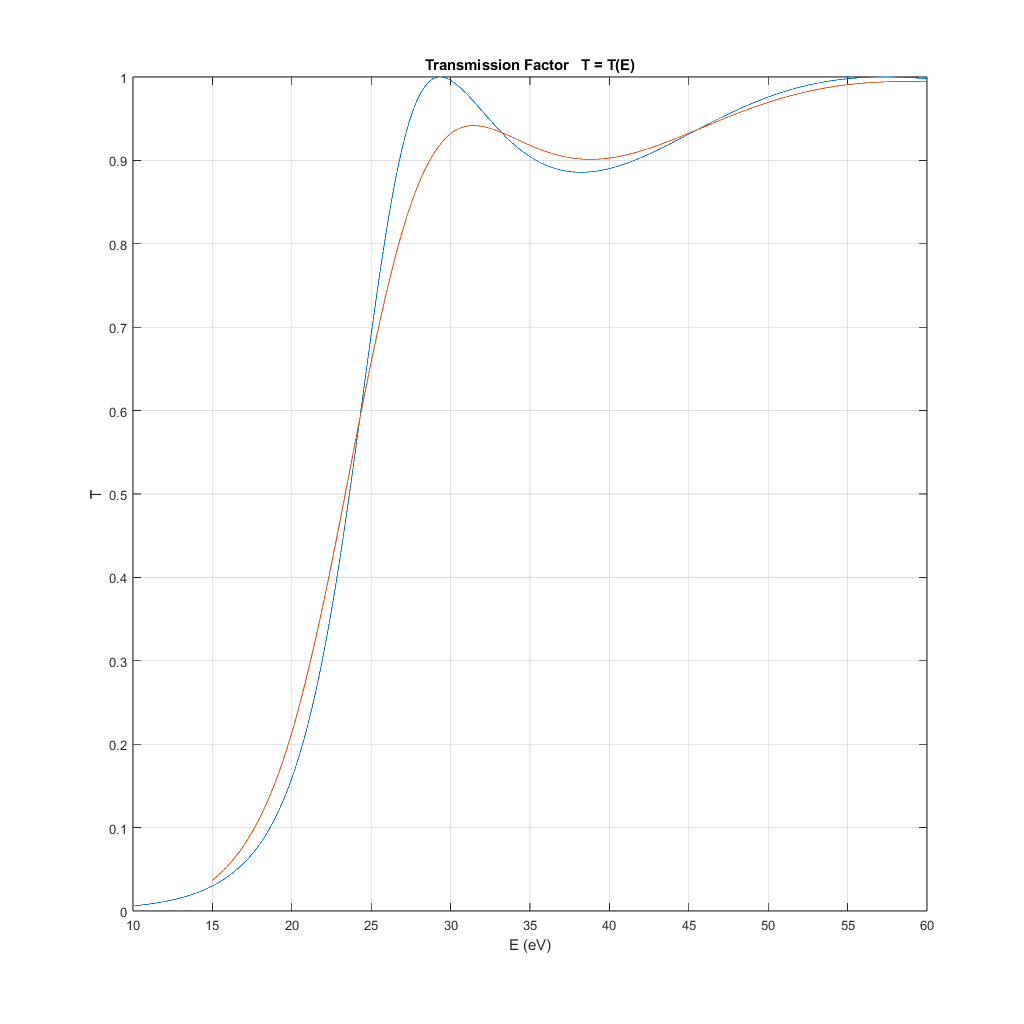
\includegraphics[width=\textwidth]{transmission_plot.png}
	\caption{Зависимость коэффициента прохождения $T$ от средней энергии электрона $E_0$}
	\label{fig:transmission}
\end{figure}

\fancyhead[L]{Задание 2} 
\section{Нахождение зависимости коэффициента прохождения $T\ $ волнового пакета от полуширины пакета $d_0$}

\subsection{Работа с программой Square\_Barrier. Получение точек для $T=T(d_0)$.}

Выставляем значения согласно варианту 
\begin{equation*}
	a = 5\text{ \AA} \quad E_0 = \Enull\text{ эВ} \quad U_0 = \Vnull\text{ эВ}
\end{equation*}
\begin{lstlisting}[language=Matlab, firstnumber=11, 
	title={\textbf{Data\_Packet.m}}, escapeinside={(*@}{@*)}]
E0 = (*@\Enull@*).;                  %energy of electron (eV)
\end{lstlisting}
\begin{lstlisting}[language=Matlab, firstnumber=16, escapeinside={(*@}{@*)}]
U0 = (*@\Vnull@*);                   %height of potential barrier (eV)
\end{lstlisting}
\begin{lstlisting}[language=Matlab, firstnumber=18, escapeinside={(*@}{@*)}]
x1 = 0;                    %coordinates of potential barrier
x2 = 5;                    %coordinates of potential barrier
\end{lstlisting}
также отодвигаем центр волнового пакета от барьера
\begin{lstlisting}[language=Matlab, firstnumber=15, title={\textbf{Data\_Packet.m}}, escapeinside={(*@}{@*)}]
x0 = -30;                  %center of wave packet (A, Angstroem)
\end{lstlisting}
Варируя значение $d_0$ 
\begin{lstlisting}[language=Matlab, firstnumber=14, 
	title={\textbf{Data\_Packet.m}}, title={\textbf{Data\_Packet.m}}, escapeinside={(*@}{@*)}]
d0 = (*@\dNull@*).;                   %half-width of wave packet (A, Angstroem)
\end{lstlisting}
в диапазоне от $2$ до $10$ \AA, фиксируем значения преодоления барьера $T$
\begin{table}[H]
	\centering
	\begin{tabularx}{\textwidth}{|C|C|C|C|C|C|C|C|C|C|}
		\hline
		$d_0$, \AA & $2$ & $3$ & $4$ & $5$ & $6$ & $7$ & $8$ & $9$ & $10$  \\
		\hline
		$T$ & $\CalcThree{\TdNullOne}$ & $\CalcThree{\TdNullTwo}$ & $\CalcThree{\TdNullThree}$ 
		    & $\CalcThree{\TdNullFour}$ & $\CalcThree{\TdNullFive}$ & $\CalcThree{\TdNullSix}$ 
			& $\CalcThree{\TdNullSeven}$ & $\CalcThree{\TdNullEight}$ & $\CalcThree{\TdNullNine}$ \\
		\hline
	\end{tabularx}
	\caption{Зависимость коэффициента прохождения $T$ от полуширины волнового пакета $d_0$}
	\label{tab:transmission_d0}
\end{table}

\subsection{Визуализация $T=T(d_0)$ и её сопоставление с теорией}

Задаём параметры для построения графика в файле
\begin{lstlisting}[language=Matlab, firstnumber=11, 
	title={\textbf{Task02.m}}, escapeinside={(*@}{@*)}]
d0 = [2 3 4 5 6 7 8 9 10];
T = [(*@{\TdNullOne}@*) (*@{\TdNullTwo}@*) (*@{\TdNullThree}@*) (*@{\TdNullFour}@*) (*@{\TdNullFive}@*) (*@{\TdNullSix}@*) (*@{\TdNullSeven}@*) (*@{\TdNullEight}@*) (*@{\TdNullNine}@*)];
\end{lstlisting}
\begin{lstlisting}[language=Matlab, firstnumber=21, escapeinside={(*@}{@*)}]
E0 = (*@\Enull@*);                    %energy of electron (eV)
\end{lstlisting}
\begin{lstlisting}[language=Matlab, firstnumber=25, escapeinside={(*@}{@*)}]
x0 = -30;                   %center of wave packet (A, Angstroem)
U0 = (*@\Vnull@*);                    %height of potential barrier (eV)
\end{lstlisting}
\begin{lstlisting}[language=Matlab, firstnumber=28, escapeinside={(*@}{@*)}]
x1 = 0;                     %coordinates of potential barrier
x2 = 5;                     %coordinates of potential barrier
\end{lstlisting}

С помощью данных из Таблицы $\ref{tab:transmission_d0}$ построим график зависимости $T$ от $d_0$ (Рис. $\ref{fig:transmission_d0}$)
\begin{figure}[H]
	\centering
	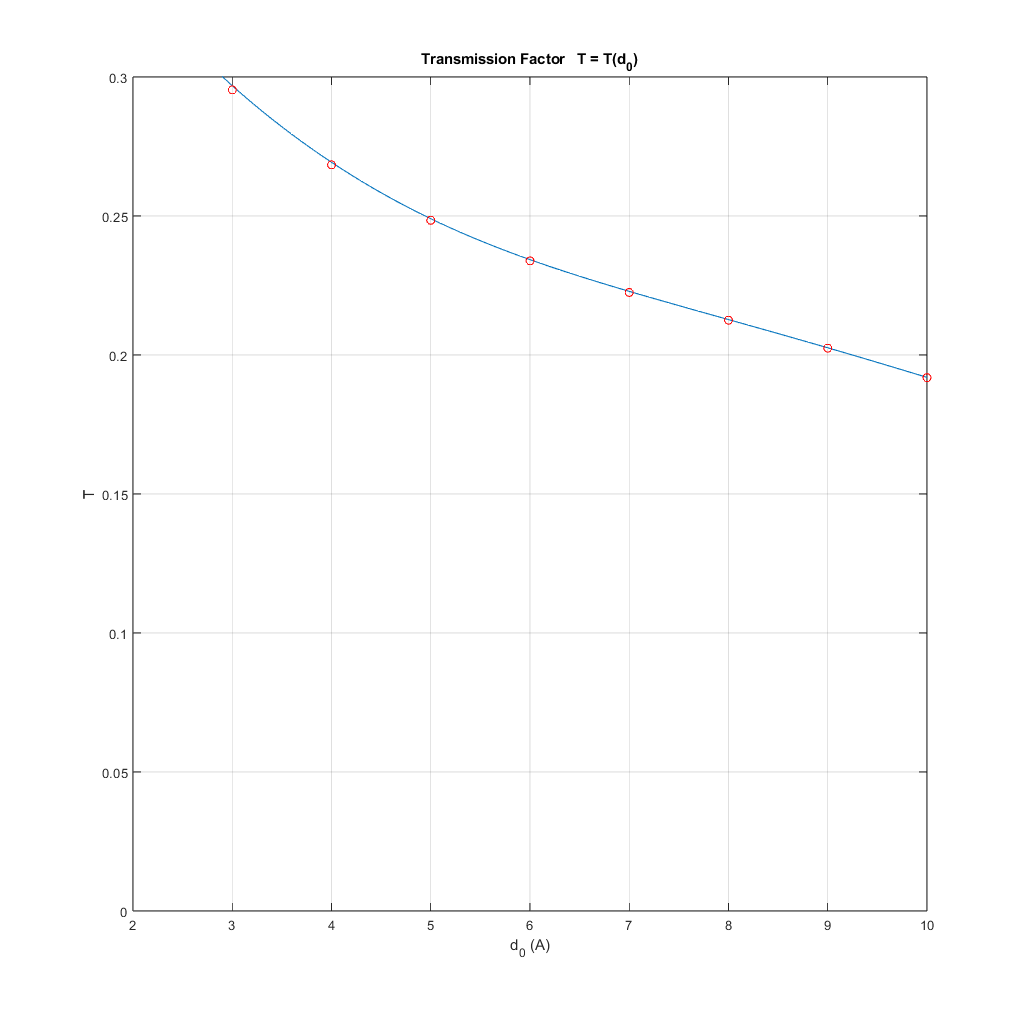
\includegraphics[width=\textwidth]{transmission_d0_plot.png}
	\caption{Зависимость коэффициента прохождения $T$ от полуширины волнового пакета $d_0$}
	\label{fig:transmission_d0}
\end{figure}
Как видно, результаты прекрасно согласуются.

\end{document}